\documentclass[oneside,10pt]{article}
\usepackage[latin1]{inputenc}
\usepackage[francais]{babel}
\usepackage[francais]{layout}
\usepackage[OT1]{fontenc}
\usepackage{listings}
\usepackage{cite}
\usepackage{textcomp}
\usepackage{graphicx}
\usepackage{mathtools}

% Reglages du document
\lstset{language=bash, frame=single, breaklines=true, basicstyle=\ttfamily, keywordstyle=\bfseries}
\setlength{\hoffset}{-18pt}        
\setlength{\oddsidemargin}{0pt} % Marge gauche sur pages impaires
\setlength{\evensidemargin}{9pt} % Marge gauche sur pages paires
\setlength{\marginparwidth}{54pt} % Largeur de note dans la marge
\setlength{\textwidth}{481pt} % Largeur de la zone de texte (17cm)
\setlength{\voffset}{-18pt} % Bon pour DOS
\setlength{\marginparsep}{7pt} % Séparation de la marge
\setlength{\topmargin}{0pt} % Pas de marge en haut
\setlength{\headheight}{13pt} % Haut de page
\setlength{\headsep}{10pt} % Entre le haut de page et le texte
\setlength{\footskip}{27pt} % Bas de page + séparation
\setlength{\textheight}{708pt} % Hauteur de la zone de texte (25cm)

\begin{document}

% Page de couverture
\title{Parall\'elisation d'un calcul et mesure de son efficacit\'e}
\author{Louis BILLIET, Florent DAVID}
\date{21 f\'evrier 2014}
\maketitle

\section{Le calcul}
Le calcul effectu\'e en parall\`ele est l'estimation de l'int\'egrale de $f(x,y)=cos(x*y)$ sur l'intervale $[0,5]^2$ selon la m\'ethode de Monte-Carlo.
L'efficacit\'e de sa parall\'elisation sera \'evalu\'ee en fonction du speed up, avec $Sp = \frac{T1}{Tp}$.
Nous avons influ\'es sur 3 param\`etres influants sur la performance : Le nombre de noeuds utili\'es pour le calcul, la taille totale du travail soumis, et la taille des chunks, les travaux soumis aux noeuds de calcul.

\section{Architecture logicielle}
L'architecture logicielle utilis\'ee est un simple ma\^itre/esclave en mode pull : les esclaves r\'eclament le travail au ma\^itre.

\section{R\'esultats relev\'es}
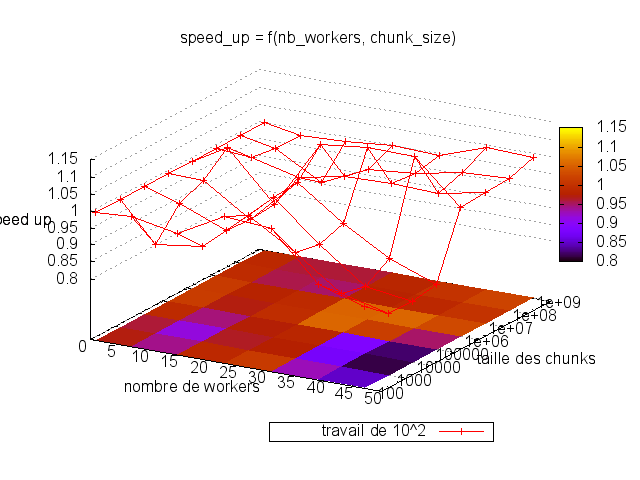
\includegraphics[scale=0.5]{travail_100.png}
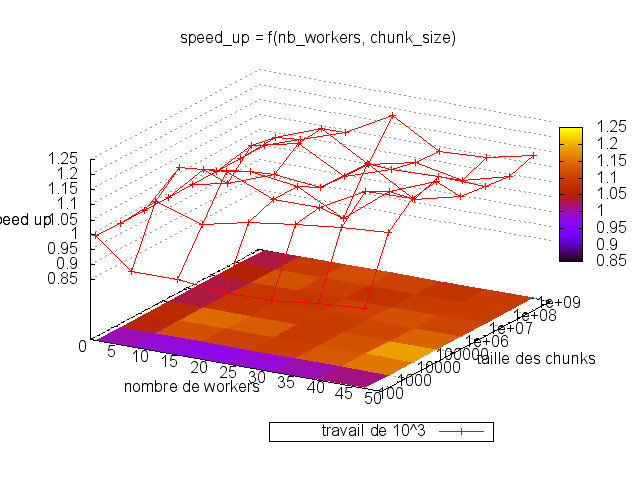
\includegraphics[scale=0.5]{travail_1000.png}
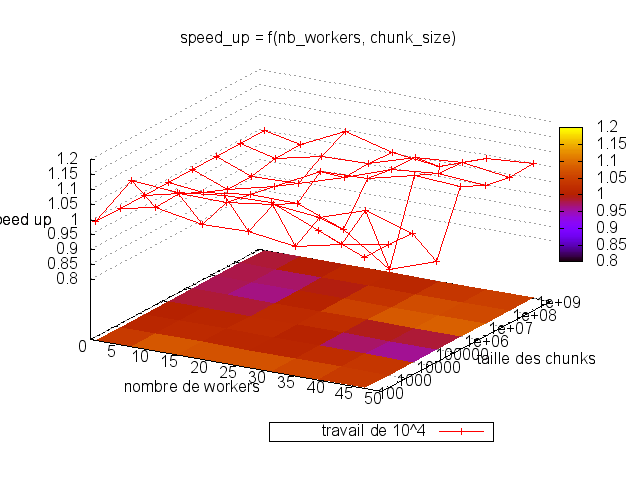
\includegraphics[scale=0.5]{travail_10000.png}
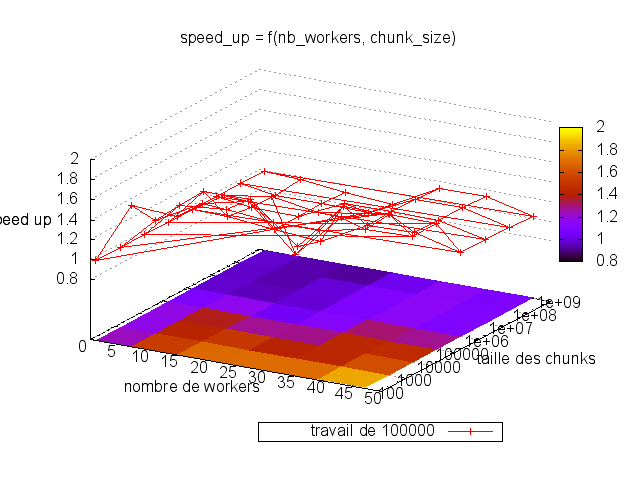
\includegraphics[scale=0.5]{travail_100000.png}
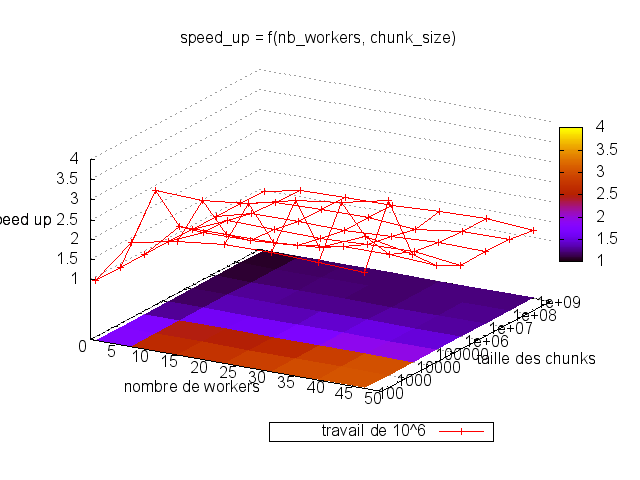
\includegraphics[scale=0.5]{travail_1000000.png}
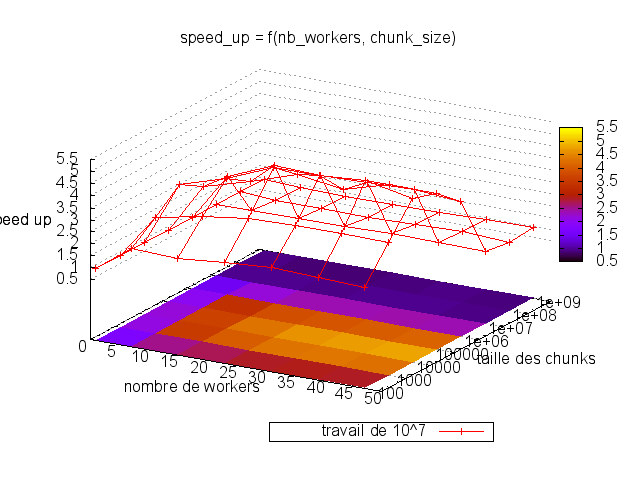
\includegraphics[scale=0.5]{travail_10000000.png}
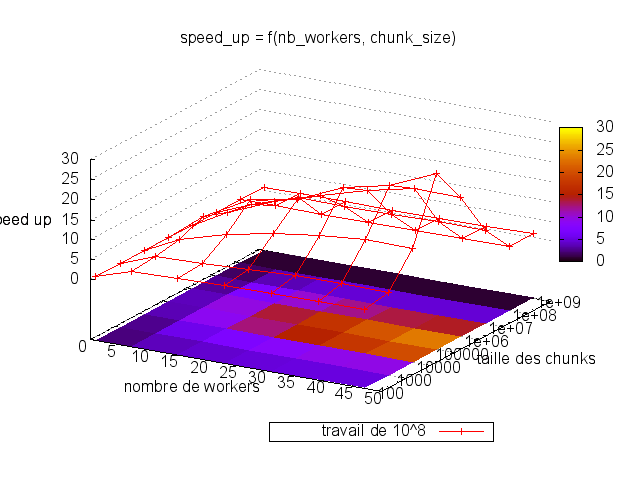
\includegraphics[scale=0.5]{travail_100000000.png}
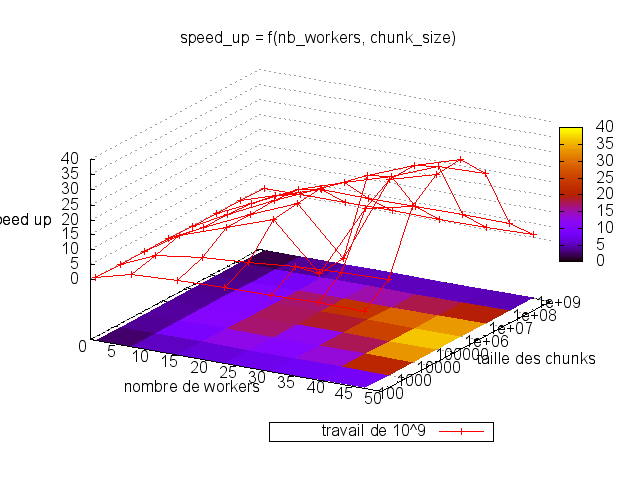
\includegraphics[scale=0.5]{travail_1000000000.png}
\section{Conclusions}

\end{document}
